\documentclass[conference]{IEEEtran}
\IEEEoverridecommandlockouts
% The preceding line is only needed to identify funding in the first footnote. If that is unneeded, please comment it out.
\usepackage{cite}
\usepackage{amsmath,amssymb,amsfonts}
\usepackage{algorithmic}
\usepackage{graphicx}
\usepackage{textcomp}
\usepackage{xcolor}
\usepackage{hyperref}
\hypersetup{
    hidelinks,
	colorlinks=true,
	allcolors=black,
	pdfstartview=Fit,
	breaklinks=true
}

\def\BibTeX{{\rm B\kern-.05em{\sc i\kern-.025em b}\kern-.08em
    T\kern-.1667em\lower.7ex\hbox{E}\kern-.125emX}}
\begin{document}

\title{\LaTeX\ Environment Configuration Under MacOS System\\
%{\footnotesize \textsuperscript{*}Note: Sub-titles are not captured in Xplore and
%should not be used}
%\thanks{Identify applicable funding agency here. If none, delete this.}
}

%\author{\IEEEauthorblockN{1\textsuperscript{st} Joker Hook}
\author{\IEEEauthorblockN{Joker Hook}
%\IEEEauthorblockA{\textit{Ocean University of China} \\
\textit{Ocean University of China}\\
Shangdong, China \\
thisemail@noreply.me}

\maketitle

\begin{abstract}
This document is a model and instructions for \LaTeX\ environment configuration under macOS system.
This document uses Visual Studio Code as a \LaTeX\ editor which you can download on the Internet freely.
This Paper is a step-by-step instruction which contains all things you will face while configuring \LaTeX\ environment.
\end{abstract}

\begin{IEEEkeywords}
environment, editor, macOS, paper, configuration
\end{IEEEkeywords}

\section{Introduction}
For researchers who need to write papers, \LaTeX\ is an indispensable weapon. 
As an editor, Word may handle basic work such as daily writing. 
However, Its internal bloated system determines the inconvenience of human use. 
We are very tired of the trouble of repeatedly modifying the font and text paragraph spacing in the process of writing in Word. 
Now It's time to switch your writing editor.
The software environment used in this article: macOS 10.15.7, VS Code, LaTeX Workshop, and MacTeX 2021.

\section{Software Installation}

\subsection{Visual Studio Installation\cite{2019Introducing}}
You can download VS Code directly on Microsoft's official website, it's convient but still do have some trouble for domestic users.
The download speed of VS Code in China is ridiculously slow. Fortunately, we do have some methods to solve this problem.
We can increase the download speed by changing the VS Code foreign mirror download address to the domestic mirror address.
Just tap this link to download \href{https://vscode.cdn.azure.cn/stable/8490d3dde47c57ba65ec40dd192d014fd2113496/VSCode-darwin.zip}{\underline{VS Code}}.

\subsection{MacTex Installation}
You can download MacTeX directly on its official \href{http://www.tug.org/mactex/mactex-download.html}{\underline{website}}.

The MacTeX installation package may be a bit big, please be patient and wait for it to finish downloading.

\subsection{LaTeX Workshop Installation}
LaTeX Workshop is a plug-in of VS code, you can download it in the VS Code plug-in store. 
After downloading LateX Workshop, you need to restart VS Code to ensure that the software uses the plug-in.

\section{Set Up VS Code}
Before you start to configure VS Code, please install it in the order of the tutorials, otherwise unnecessary trouble will occur.

\subsection{Open Setting.json File}\label{AA}
On the VS Code interface, tap the gear mark in the lower left corner, and then select the setting column in the pop-up candidate box.

After opening the settings, type the “tool” keyword in the search bar and search, find the LateX option in the extension column and choose it. 
Find the “Latex-workshop>Latex:Tools” option in the right area, and tap the link “Edit in setting.json” below to open the editing interface. 
The setting window shows on Fig. 1.

\begin{figure}[htbp]
    \centerline{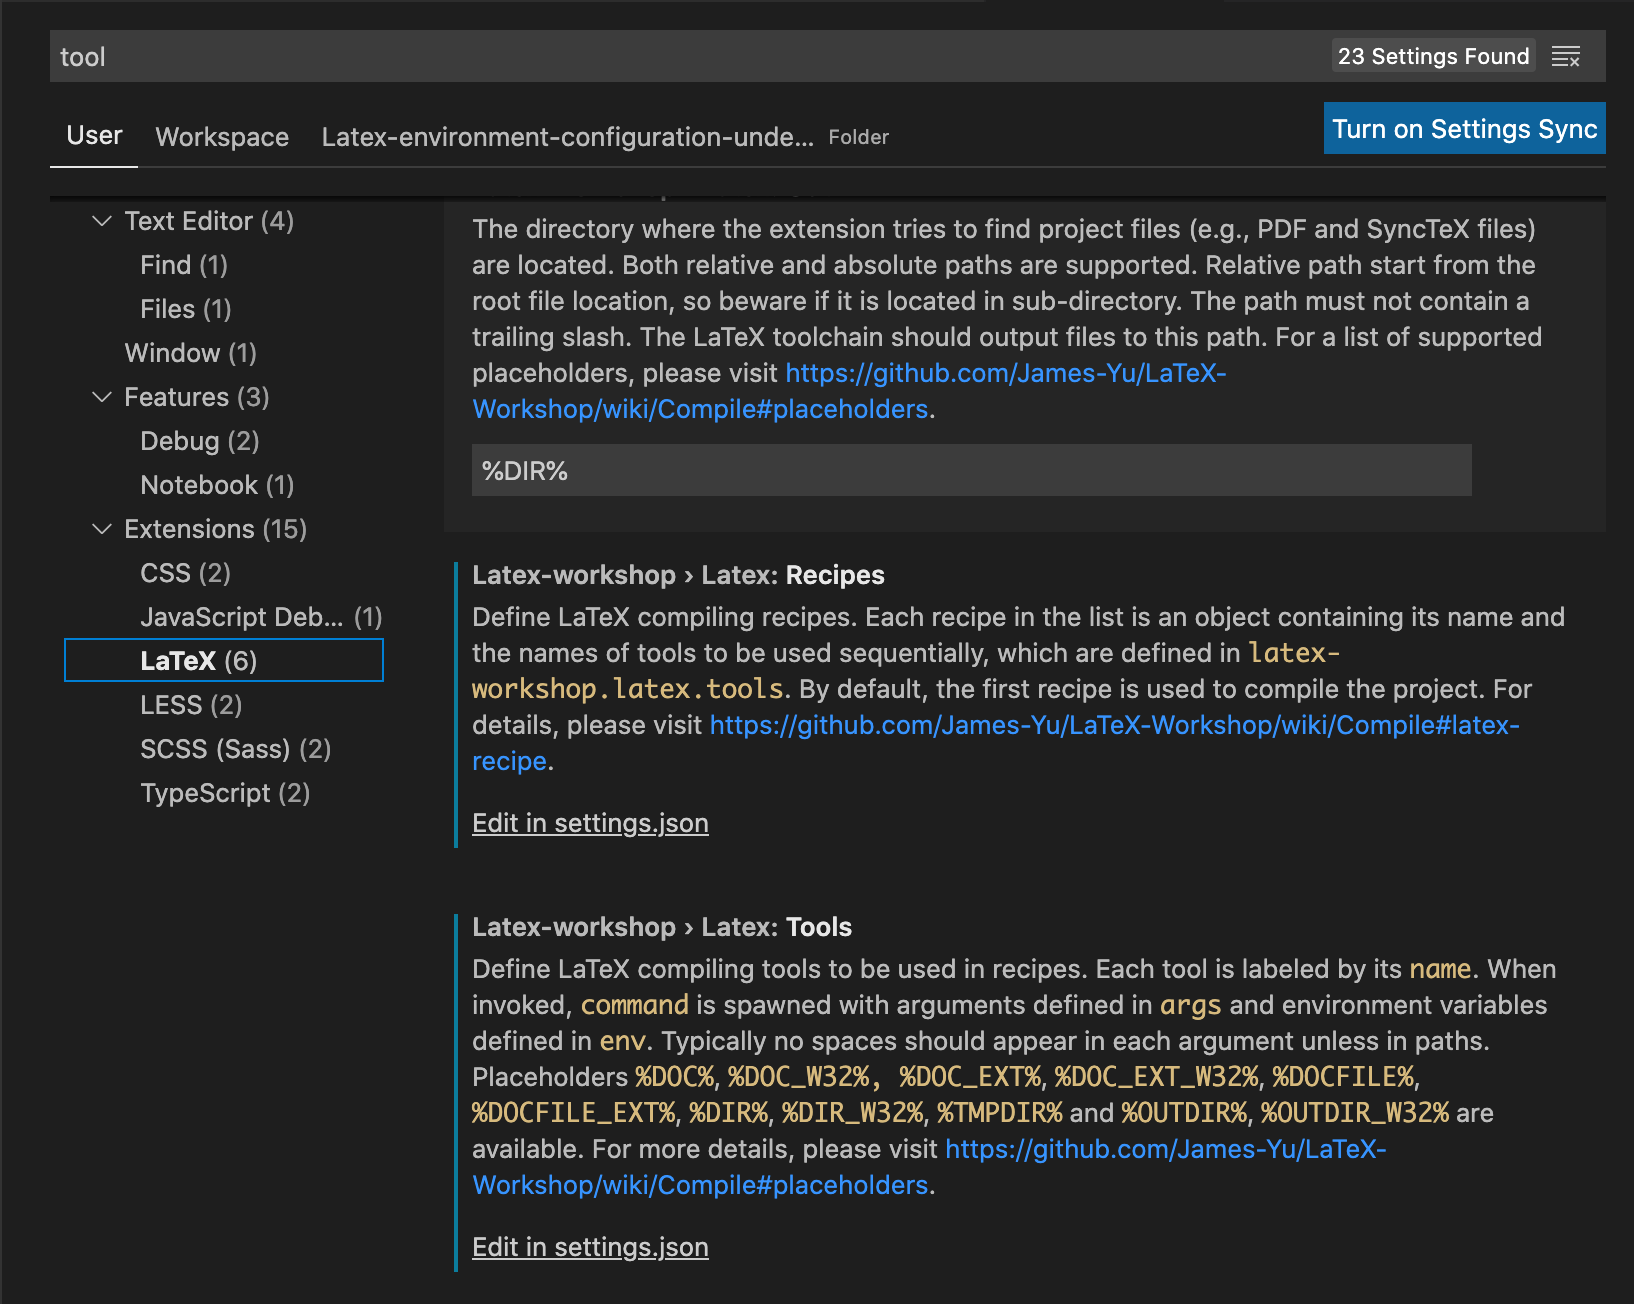
\includegraphics[width=0.49\textwidth]{show_tools.png}}
    \caption{Edit in setting.json}
    \label{fig1}
\end{figure}

\subsection{Support Chinese format}
Professor Gartner invented Tex in order to make the typesetting of his masterpiece ``Computer Programming Art'' more beautiful. 
But he did not consider the use environment of Chinese, 
fortunately the underlying interface was implemented very well, 
making it later implement the corresponding interface to support Chinese.

First of all, you need to add the following codes to ``latex-workshop.latex.tools" which locates in the setting.json file you have opened.
The default compilation method of latex-workshop is latexmk, which does not support Chinese preview. 
The xelatex compilation method uses utf-8 encoding, which supports Chinese. 
As long as the font is selected, you can directly compile and display Chinese characters in the document.

\begin{figure}[htbp]
    \centerline{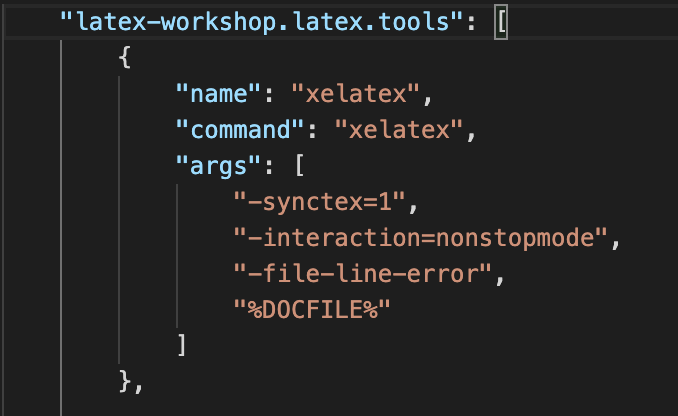
\includegraphics[width=0.49\textwidth]{tool_xelatex.png}}
    \caption{Codes for tools}
    \label{fig2}
\end{figure}

Repeat the above methods, 
search for recipes in the settings interface, 
find Latex-workshop>Latex:Recipes, 
and enter the settings.json file again. 
In latex-workshop.latex.recipes, 
you can see the default four compilation methods of Latex Workshop. 
Add the following codes before the first compilation method.

\begin{figure}[htbp]
    \centerline{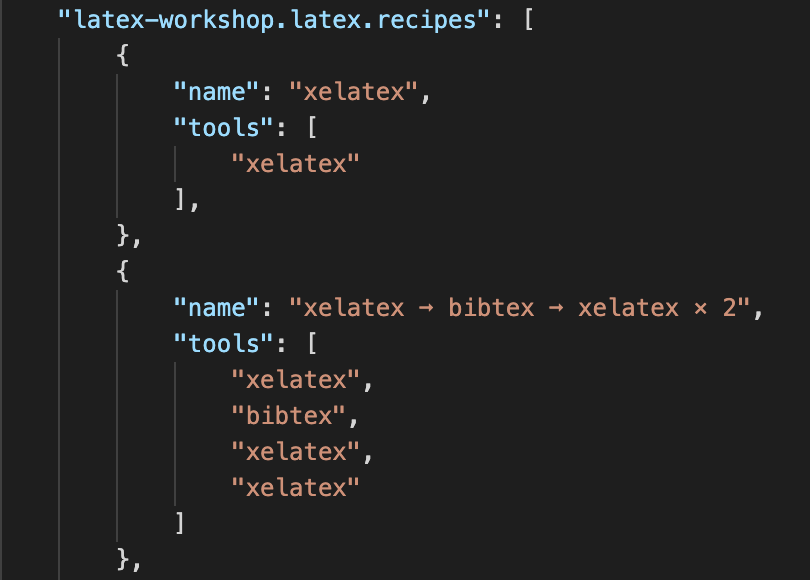
\includegraphics[width=0.49\textwidth]{recipes_confi.png}}
    \caption{Codes for recipes}
    \label{fig3}
\end{figure}

After add those codes to ``latex-workshop.latex.recipes", 
comment out the three compilation methods just below the methods you have added.

Now save the files you have changed before, 
then restart VS Code, 
those modified configurations can now be used normally.

\section{An Example of Using \LaTeX}
After configuring the LateX environment, 
you can start editing the first text. 
For convenience, 
first download the \href{https://www.elsevier.com/authors/author-schemas/latex-instructions}{\underline{Elsevier template}} used in this example on the Elsevier official website.

\subsection{VS Code Workspace}
Now open VS Code, choose "File->Add Folder to Workspace" on the menu, then choose the elsarticle-template files you have just downloaded.
You will find that there are many files in the folder. 
We only care about the file which ends in .tex, it's the file you use for writing.

The above steps are designed to teach you how to add folders to the workspace in VS Code, 
and the files in the workspace can be compiled normally in VS Code. 
For more tips on using VS Code, 
ou can find it on the \href{https://code.visualstudio.com/learn}{\underline{VS Code official website}}.

\subsection{Compile \LaTeX\ Files}
Select elsarticle-template.tex file, you will find that there is an extra TEX icon in the left border of VS Code.
Tap on the icon, and you will find a menu which contains three columns named "COMMANDS", "STRUCTURE", "SNIPPED VIEW".

Focus on the "COMMANDS" column, tap the button "Build LaTeX project", and you will find there are so many different recipes.
Just tap the first recipe: "Recipe:xelatex", then select the "View LaTeX PDF" column, and choose "View in VS Code tab".
Now you will see the compiled PDF file.

% \begin{figure}[htbp]
%     \centerline{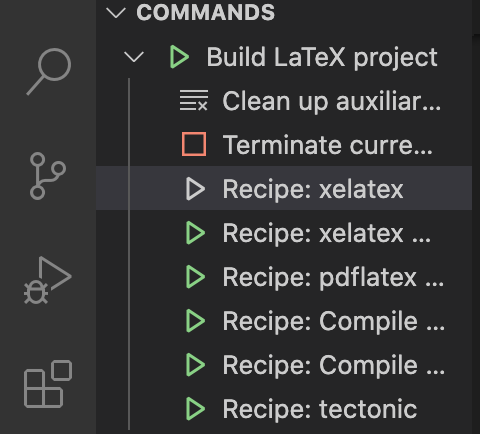
\includegraphics[width=0.47\textwidth]{COMMANDS.png}}
%     \caption{The COMMANDS column}
%     \label{fig4}
% \end{figure}



% \begin{thebibliography}{00}
%     \bibitem{b1} G. Eason, B. Noble, and I. N. Sneddon, ``On certain integrals of Lipschitz-Hankel type involving products of Bessel functions,'' Phil. Trans. Roy. Soc. London, vol. A247, pp. 529--551, April 1955.
    
% \end{thebibliography}
\bibliographystyle{ieeetr}
\bibliography{Intro_VScode}
\end{document}
